\documentclass[aspectratio=169, t, 8pt]{beamer}

%------configurando acentos-----------
\usepackage[utf8]{inputenc}
\usepackage[brazil]{babel}

%-------Estilos Beamer---------------
\usetheme{Frankfurt}
\usecolortheme{whale}
\usefonttheme{serif}

\linespread{1.2}

%--------Dados do Documento
\title{Matemática: Lista de Exercícios}
\author{prof. Eduardo}
\institute{Pré-Universitário Oficina do Saber / UFF}
\date{\today}


%-------- Pacotes Matemática -------------
\usepackage{amsmath}
\usepackage{amsthm}
\usepackage{amsfonts}
\usepackage{amssymb}
\usepackage{xfrac}
\usepackage{thmtools}

%-------- Configuração Listas---------
\usepackage{enumitem}

\setcounter{tocdepth}{2}

\newcounter{questaovest}
\newcommand{\vest}[1]{\stepcounter{questaovest}\item[\textbf{Questão \arabic{questaovest}} (#1):]}
\setlist[enumerate]{
    align=left,
    leftmargin=1.8em,
    itemindent=1.8em
    }

\setlist[enumerate,2]{
    label=\alph*.,
    font=\bfseries,
    itemsep=0.1pt,
    labelsep=0em,
    parsep=0pt,
    leftmargin=0em
    }

%------------- Atalho para imagens ------------
\graphicspath{{./src/img/}}


\begin{document}

    \begin{frame}
        \titlepage
    \end{frame}
   
    \begin{frame}
        \frametitle{Funções}
        
        \begin{enumerate}
            \vest{ENEM}Um laticínio possui dois reservatórios de leite. Cada reservatório é abastecido por uma torneira acoplada a um tanque resfriado. O volume, em litros, desses reservatórios depende da quantidade inicial de leite no reservatório e do tempo $t$, em horas, em que as duas torneiras ficam abertas. Os volumes são dados pelas funções $V_1(t) = 250t^3 - 100t + 3000$ e $V_2(t) = 150t^3 + 69t + 3000$
            
            Depois de aberta cada torneira, o volume de leite de um reservatório é igual ao do outro no instante $t = 0$ e, também, no tempo $t$ igual a:
            \vspace{1em}
            \begin{enumerate}
                \item 1,3 h
                \item 1,69 h
                \item 10 h
                \item 13,0 h
                \item 16,9 h
            \end{enumerate}

        \end{enumerate}
    \end{frame}

    \begin{frame}
        \frametitle{Funções}
        \begin{enumerate}
            \vest{ENEM} Em fevereiro, o governo da Cidade do México, metrópole com uma das maiores frotas de automóveis do mundo, passou a oferecer à população bicicletas como opção de transporte. Por uma anuidade de 24 dólares, os usuários têm direito a 30 minutos de uso livre por dia. O ciclista pode retirar em uma estação e devolver em qualquer outra e, se quiser estender a pedalada, paga 3 dólares por hora extra.

            \hfill {\footnotesize Revista Exame. 21 abr. 2010.}
            
            \vspace{1em}
            A expressão que relaciona o valor $f$ pago pela utilização da bicicleta por um ano, quando se utilizam $x$ horas extras nesse período é:

            \vspace{1em}
            \begin{enumerate}
                \item $f(x) = 3x$
                \item $f(x) = 24$
                \item $f(x) = 27$
                \item $f(x) = 3x + 24$
                \item $f(x) = 24x + 3$
            \end{enumerate}
        \end{enumerate}
    \end{frame}

    \begin{frame}
        \frametitle{Teoria dos Conjuntos}
        \begin{enumerate}
            \vest{UFRN-2001}Uma pesquisa de opinião, realizada num bairro de Natal, apresentou o resultado seguinte: 65\% dos entrevistados frequentavam a praia de Ponta Negra, 55\% frequentavam a praia do Meio e 15\% não iam à praia.
            
            De acordo com essa pesquisa, o percentual dos entrevistados que frequentavam ambas as praias era de:
            \vspace{1em}
                \begin{enumerate}
                    \item 20\%
                    \item 35\%
                    \item 40\%
                    \item 25\%
                \end{enumerate}
        \end{enumerate}
    \end{frame}

    \begin{frame}
        \frametitle{Sistema de Equações}
        \begin{enumerate}
            \vest{IFAL-2023} Um jogo de cara ou coroa tinha a seguinte regra: quando o lado da moeda era cara, o jogador ganhava 3 pontos e, quando era coroa, o jogador ganhava apenas 1 ponto. Após lançar a moeda 10 vezes, um determinado jogador obteve 24 pontos. Quantas vezes, nesses 10 lançamentos, saiu o lado cara da moeda para esse jogador?
            \vspace{1em}
            \begin{enumerate}
                \item 3
                \item 4
                \item 5
                \item 6
                \item 7
            \end{enumerate}
        \end{enumerate}
    \end{frame}

    \begin{frame}
        \frametitle{Geometria}
        \begin{enumerate}
            \vest{CESGRANRIO} Certa noite, uma moça, de 1,50 m de altura, estava a dois metros de distância de um poste de luz de 4 m de altura. O comprimento da sombra da moça no chão era de:
            \vspace{1em}
            \begin{enumerate}
                \item 0,75 m
                \item 1,20 m
                \item 1,80 m
                \item 2,40 m
                \item 3,20 m
            \end{enumerate}
        \end{enumerate}
    \end{frame}

    \begin{frame}
        \frametitle{Geometria}
        \begin{enumerate}
            \vest{ULBRA-2016}A figura a seguir representa um cubo de lado medindo 6 cm e um triângulo ABC. A área desse triângulo mede?
            \begin{figure}[!htbp]
                \raggedright
                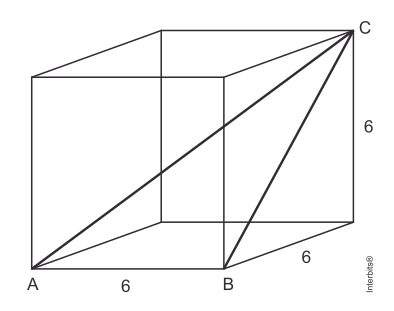
\includegraphics[width=0.32\textwidth]{figura01.png}  
            \end{figure}

            \begin{enumerate}
                \item $36\sqrt{2} cm^2$
                \item $18\sqrt{2} cm^2$
                \item $24\sqrt{2} cm^2$
                \item $12\sqrt{2} cm^2$
                \item $6\sqrt{2} cm^2$
            \end{enumerate}
        \end{enumerate}
    \end{frame}
\end{document}